\documentclass[12pt, a4paper]{article}

\usepackage[utf8]{inputenc}
\usepackage[T1]{fontenc}
\usepackage[russian]{babel}
\usepackage[oglav,spisok,boldsect,eqwhole,figwhole,hyperref,hyperprint,remarks,greekit]{./style/fn2kursstyle}
\graphicspath{{./style/}{./figures/}}
\usepackage{caption}
\usepackage{subcaption}
\usepackage{adjustbox}
\usepackage{multirow}
\usepackage{supertabular}
\usepackage{multicol}

\usepackage{diagbox}
\usepackage{listings}
\usepackage{color}

\definecolor{dkgreen}{rgb}{0,0.6,0}
\definecolor{gray}{rgb}{0.5,0.5,0.5}
\definecolor{mauve}{rgb}{0.58,0,0.82}

\lstset{frame=tb,
	inputencoding=utf8,
	basicstyle=\ttfamily,
	extendedchars=\true,
	showspaces=\false,
	showstringspaces=\false,
	language=Python,
	aboveskip=3mm,
	belowskip=3mm,
	showstringspaces=false,
	columns=flexible,
	basicstyle={\small},
	numbers=left,
	numberstyle=\tiny\color{gray},
	keywordstyle=\color{red},
	commentstyle=\color{dkgreen},
	stringstyle=\color{mauve},
	breaklines=true,
	breakatwhitespace=true,
	tabsize=3
}







\renewcommand{\phi}{\varphi}

\renewcommand{\kappa}{\varkappa}



\title{	`}
\author{О.\,Д.~Климов}
\supervisor{М.\,П.~Галанин}
\group{ФН2-71Б}
\date{2024}

\renewcommand{\labelenumi}{\theenumi)}
\begin{document}

\maketitle
\tableofcontents
\clearpage

\section-{Введение}
Технологиям нейронных сетей можно найти применение в совершенно разных прикладных задачах науки и техники. Например, в задаче восстановления графика решений уравнения по неточно заданным данных о решениях. В силу нелинейности распознавания изображений нахождение точных алгоритмов для такой задачи испытывало ряд трудностей. Однако с развитием программирования и вычислительной техники стало возможным решать данную задачу методами нейронных сетей.

\section{Постановка задачи}

\subsection{Формулировка}
Необходимо для одномерного уравнения переноса реализовать и протестировать алгоритм улучшения решения на основе искусственных нейронных сетей. Для анализа работы программы использовать систему из 5 тестов: левый и правый треугольники, прямоугольник, косинус, зуб.  

\begin{figure}[!hp]
	\centering
	\begin{tabular}{ccccc@{\hspace{0.5cm}}ccccc}
		\begin{subfigure}[t]{0.19\textwidth}
			\centering
			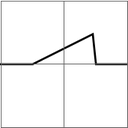
\includegraphics[width=\textwidth]{1}
			\caption{Тест 1}
			\label{test1}
		\end{subfigure} &
		\begin{subfigure}[t]{0.19\textwidth}
			\centering
			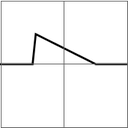
\includegraphics[width=\textwidth]{2}
			\caption{Тест 2}
			\label{test2}
		\end{subfigure} & 
		\begin{subfigure}[t]{0.19\textwidth}
			\centering
			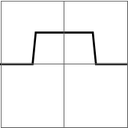
\includegraphics[width=\textwidth]{3}
			\caption{Тест 3}
			\label{test3}
		\end{subfigure} &
		\begin{subfigure}[t]{0.19\textwidth}
			\centering
			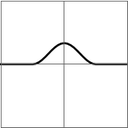
\includegraphics[width=\textwidth]{4}
			\caption{Тест 4}
			\label{test4}
		\end{subfigure} &
		\begin{subfigure}[t]{0.19\textwidth}
			\centering
			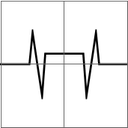
\includegraphics[width=\textwidth]{5}
			\caption{Тест 5}
			\label{test5}
		\end{subfigure} 
	\end{tabular}
	\caption{Система тестов}
	\label{primer_nabor}
\end{figure}
\subsection{Пояснения}
Рассмотрим задачу Коши для одномерного уравнения переноса следующего вида:
\begin{equation}
	\begin{cases}
		\dfrac{\partial u}{\partial t} + a\dfrac{\partial u}{\partial x} = 0, \\
		u(x, 0) = u_0(x),
	\end{cases} 
	\text{где } \quad a = const > 0, \quad t \in (0, T), \quad x \in (-\infty, +\infty) .
\end{equation}

Приведем аналитическое решение. Уравнение можно записать в виде $ u_t + a u_x = 0 $.
Запишем и решим характеристическое уравнение:
\begin{equation*}
	\dfrac{dt}{1} = \dfrac{dx}{a} = \dfrac{du}{0} \quad \implies  \quad 
	\begin{cases}
		u = C_1,\\
		x = a t + C_2
	\end{cases} 
	\quad \implies \quad
	\begin{cases}
		C_1 = u,\\
		C_2 = x - at
	\end{cases}
	\quad \implies \quad
	u = \psi(x-a t).
\end{equation*}
\newpage
Применим граничные условия:
\vspace{-1em}
\begin{equation*}
	u(x, 0) = u_0(x),
	\quad \implies \quad
	\psi(x) = u_0(x),
	\quad \implies \quad
	u = u_0(x-a t).
\end{equation*}

Получим аналитическое решение уравнения $u = u_0(x-at)$. Решение заключается в сносе неизменного профиля по характеристикам. 

Важнейшим свойством рассматриваемого решения будет являться сохранение начального профиля: если начальное решение представляет собой, например, профиль буквы «М», то оно будет сохранять его таким всегда. 

Разностные схемы, аппроксимирующие такое уравнение, в той или иной степени искажают точное решение. Выделяют два эффекта потери формы --- \textbf{диссипацию} и \textbf{дисперсию}.

Дисперсия возникает, когда различные гармонические компоненты волны (с различными частотами) распространяются с разными фазовыми скоростями. В результате форма волны искажается: волновой фронт "растягивается" или "смещается". Так появляются ложные осцилляции (колебания) вокруг резких границ волнового фронта. \cite[c.283]{1}

Диссипация описывает процесс затухания волнового сигнала из-за рассеивания энергии. Она возникает при использовании схем с ненулевой вязкостью, из-за чего искажается амплитуда волны.  

\vspace{-2em}
\begin{figure}[!h]
	\centering
	\begin{subfigure}[t]{0.45\textwidth}
		\centering
		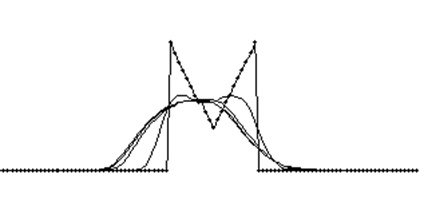
\includegraphics[width=\textwidth]{prim1}
		\caption{Пример схемы с диссипацией}
	\end{subfigure}
	\quad\quad\quad
	\begin{subfigure}[t]{0.45\textwidth}
		\centering
		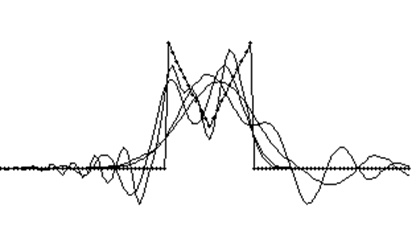
\includegraphics[width=\textwidth]{prim2}
		\caption{Пример схемы с дисперсией}
	\end{subfigure}
	\caption{Пример точного (буква М) и численного решения уравнения переноса при некоторых различных числах Куранта. Иллюстрации взяты из \cite[c.416]{1}} .
\end{figure}
\vspace{-2em}
Задачей является исправление и приведение решения уравнения к менее искаженному виду. В силу особенностей выбранного алгоритма далее ограничимся слабым смещением и растяжением решения, таким, чтобы различить зрительно. 

\newpage

\section{Технологии нейронных сетей}
Для решения поставленной задачи обратимся к теории нейронных сетей. В следующих пунктах представлены общие идеи традиционных алгоритмов сетей. Также отдельно рассмотрен алгоритм сверточной нейронной сети.
\subsection{Понятие нейронной сети}
\textbf{Нейронная сеть} --- это алгоритм основанный на принципе организации биологических нейронных сетей, т.е. лежащих в основе живых существ. Сам этот алгоритм можно интерпретировать совершенно по-разному.

С математической точки зрения, нейронная сеть представляет собой математическую модель, которая соответствует некому процессу взаимодействия вычислительных блоков (нейронов). В нее входит многопараметрическая задача нелинейной оптимизации, появляющейся при установлении параметров сети.\cite{3}

Также имеет место другой взгляд на математическую интерпретацию. Нейронную сеть можно рассматривать как нелинейное преобразование входного вектора, которое получается композицией всех функций сети(нейронов). Нелинейность получается за счет наличия нелинейных функций активации в каждом нейроне.

С точки зрения программирования, нейронная сеть представляет собой результат эволюции алгоритмов решения алгоритмически сложных задач с обработкой большого объема входных данных, а также возможность интеграции ускорителей вычислений (GPU, TPU). Именно здесь появляется связь нейронных сетей с машинным обучением. 

\textbf{Машинное обучение} - это область компьютерных наук, к которой относят новую парадигму программирования, где на вход программы поступают данные и ответы, соответствующие этим данным, а результатом получается правила, которые можно применить к новым данным для получения оригинальных ответов. То есть в этой парадигме система обучается, в то время как в классическом программировании в программу вводятся правила и данные для обработки и получают ответ. Таким образом нейронные сети это один из подходов в рамках машинного обучения. \cite[c.28]{9}

Стоит отметит, что также отдельно выделяют область \textbf{глубокого обучения}, к которой относят нейронные сети с большим количеством слоев. В определенных случаях увеличение количества слоев сети приводит яркому развитию ее способностей к понимаю данных. \cite[c.31]{9}

Далее будем нейронную сеть будем рассматривать в виде приближенной математической модели, описывая включенные в нее алгоритмы. 

\subsection{Нейрон}
\textbf{Нейрон} --- единица обработки информации в нейронной сети. Он представляет из себя элемент, который вычисляет выходной сигнал из совокупности входных сигналов по определенному правилу. На блок-схеме рис. \ref{neiron} показана модель нейрона, лежащего в основе искусственных нейронных сетей \cite[c.28]{7}. 

\begin{figure}[!h]
	\centering
	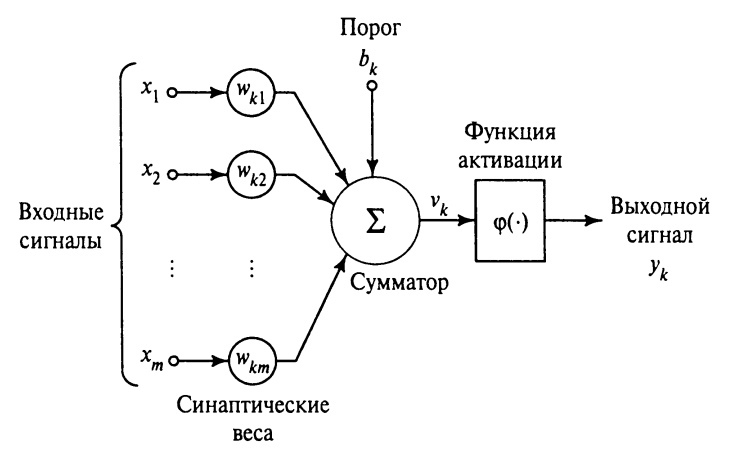
\includegraphics[width=0.8\linewidth]{neiron}
	\caption{Нелинейная модель $k$-го нейрона}
	\label{neiron}
\end{figure}

В этой модели выделяют три основных элемента:
\begin{itemize}
	\item \textbf{Набор связей}, каждый из которых характеризуется своим весом(силой). В частности, сигнал $x_j$ на входе связи $j$, связанного с нейронном $k$, умножается на вес $w_{kj}$(первый индекс относится к рассматриваемому нейрону, а второй ко входному окончанию связи). Вес может иметь как положительные так и отрицательные значения.
	\item \textbf{Сумматор} складывает входные сигналы, взвешенные относительно соответствующих связей нейрона. Эту операцию можно описать как линейную комбинацию.
	\item \textbf{Функция активации} ограничивает амплитуду выходного сигнала нейрона. Обычно нормализованный диапазон амплитуд выхода нейрона лежит в интервале $[0, 1]$ или $[-1, 1]$.
	\item \textbf{Пороговый элемент} $b_k$, который отражает увеличение или уменьшение входного сигнала на функцию активации.
\end{itemize}

\newpage
В математическом представлении функционирование нейрона $k$ можно описать следующей парой уравнений
\begin{equation}
	y_k = \phi(u_k + b_k), \quad u_k = \sum_{j = 1}^{m} w_{kj}x_j 
	\label{1}
\end{equation}
где $x_1, x_2, \dots, x_m$ --- входные сигналы,
$w_{k1}, w_{k2}, \dots, w_{km}$ --- веса связей нейрона $k$, \\
$u_k $ --- линейная комбинация входных воздействий,
$b_k$ --- порог,\\
$ \phi(\dot) $ --- функция активации,
$ y_k $ --- выходной сигнал.

Использование порога $b_k$ обеспечивает эффект аффинного преобразования выхода линейного сумматора $u_k$. В частности, в зависимости от того, какое значение принимает порог,  положительное или отрицательное, можно двигать значения выхода нейрона. Обозначим $w_{k0} = b_k$ и преобразуем модель к следующему виду
\begin{equation}
	y_k = \phi(v_k), \quad v_k = \sum_{j = 0}^{m} w_{kj}x_j 
	\label{2}
\end{equation}
 Таким образом, в выражении \eqref{2} добавился новый синапс. Его входной сигнал и вес соответственно равны
 \begin{equation*}
 	x_0 = +1, \quad w_{k0} = b_k.
 \end{equation*}
 Это позволило трансформировать модель нейрона к виду, при котором добавляется новый входной сигнал фиксированной величины $+1$, а также появляется новый синаптический вес, равный пороговому значению $b_k$. Хотя на первый взгляд кажется, что такая модель \eqref{2} отличается от изначальной \eqref{1}, математически они эквивалентны.
  
  
  
%\newpage
\subsection{Структура сети}

В нейронной сети нейроны упорядочено располагаются по слоям и связываются между собой  направленными связями. Каждый нейрон принимает входные сигналы от нейронов предыдущего слоя, преобразует их с помощью весов и функции активации и передает результат на следующий слой.  Принято разделять три ключевых типа слоев: входной, скрытые и выходной слои.

\textbf{Входной слой} служит для приема исходных данных.  Входной слой не выполняет вычислений и лишь передает данные на первый скрытый слой. Каждый нейрон этого слоя соответствует одному из признаков входного вектора
  \begin{equation}
 	 x = (x_1, x_2, ..., x_m).
 	 \label{3}
 \end{equation}

\textbf{Скрытые слои} --- это промежуточные слои между входным и выходным слоями. Они выполняют основную обработку информации и могут включать несколько уровней, каждый из которых преобразует данные через нелинейные функции активации.

\textbf{Выходной слой} производит итоговый результат работы сети. Кол-во нейронов в этом слое зависит исключительно от задачи. Как результат мы получаем 
  \begin{equation}
	y = (y_1, y_2, ..., y_k).
	\label{4}
\end{equation}


 \textbf{Глубина} сети определяется числом скрытых слоев, а \textbf{ширина} — количеством нейронов в каждом слое.  Добавляя один или несколько скрытых слоев, мы можем выделить  из входных данных закономерности более высокого порядка. 
 
 Архитектуру сети определяют связи между слоями. Существует множество вариантов расположить связи в сети, наиболее значимыми являются:
 \begin{itemize}
 	\item \textbf{Полносвязная сеть} --- каждый нейрон одного слоя соединен со всеми нейронами следующего.
 	\item \textbf{Сверточные сети} --- связи устанавливаются между локальными группами нейронов для анализа пространственных структур данных.
 	\item \textbf{Рекуррентные сети} --- связи могут иметь обратную направленность для учета временной зависимости. 
 \end{itemize}
  
 %\newpage
\subsection{Обучение}
\textbf{Обучением нейронной сети} называется процесс настройки весов $w_{ij}$ таким образом, чтобы сеть могла эффективно выполнять поставленную задачу. Обучение основано на минимизации ошибки между предсказанным выходом сети и целевыми значениями на обучающем наборе данных. Рассмотрим исключительно тип обучения с учителем, где нам известны целевые значения на входные данные. \cite{2}

Сначала происходит инициализация параметров случайными значениями с использованием специальных методов. Производят прямое распространение --- входные данные $x = (x_1, x_2, ..., x_m)$ передаются на вычисления в сеть. После выход последнего слоя $y_{pred}$ сравнивается с целевым значением $y_{true}$.

Для сравнения $y_{pred}$ и $y_{true}$ вводят понятие \textbf{функции потерь} $L$, которая измеряет ошибку сети. Ее выбор зависит от типа задачи, часто используют \textbf{среднеквадратическую ошибка (MSE)}:
\begin{equation}
	L = \frac{1}{n} \sum_{i=1}^{n} (y_{pred, i} - y_{true, i})^2,
\end{equation}


Одним из фундаментальных и наиболее часто применимых подходов к обучению сети является \textbf{метод обратного распространения ошибки}. Этот метод позволяет вычислить градиенты функции потерь по каждому параметру сети, используя правило цепочки для передачи ошибки от выходного слоя к предыдущим слоям.

Алгоритм следующий:
\begin{enumerate}
	\item Прямое распространение: вычисление выходных значений нейронов и функции потерь.
	\item Обратное распространение: вычисление частных производных функции потерь по параметрам сети.
	\item Обновление параметров с использованием метода оптимизации (например, градиентного спуска).
\end{enumerate}

Согласно соотношению \eqref{2} на каждом нейроне $k$ вычисляется взвешенная сумма входов $u_k = \sum_{j=0}^{m} w_{kj} x_j$ и его активация с использованием функции активации $\phi$.

Для вычисления ошибки на выходном слое используется частная производная функции потерь $L$ по выходному значению $y_k$
\begin{equation}
	\delta_k = \frac{\partial L}{\partial y_k} \cdot \phi'(u_k),
	\label{7}
\end{equation}
где $\phi'(u_k)$ — производная функции активации.

Ошибка передается обратно через связи, корректируя веса на каждом слое:
\begin{equation}
	\delta_j = \sum_{k=1}^{n} \delta_k w_{kj} \cdot \phi'(u_j),
	\label{8}
\end{equation}
где $n$ — количество нейронов следующего слоя.

Частные производные функции потерь по весам и смещениям вычисляются следующим образом
\begin{equation}
	\frac{\partial L}{\partial w_{kj}} = \delta_k \cdot x_j,
\end{equation}

Для обновления параметров используется метод градиентного спуска\cite[c.23]{10}
\begin{equation}
	w_{kj} \leftarrow w_{kj} - \eta \cdot \frac{\partial L}{\partial w_{kj}},
	\label{11}
\end{equation}
где $\eta$ — скорость обучения.

Таким образом, метод обратного распространения ошибки позволяет сети корректировать свои параметры, постепенно минимизируя ошибку на входных данных. После повторения описанных шагов для определенного набора входных данных сеть настраивает свои параметры, чтобы лучше обобщать на новых данных.

\newpage
\subsection{Применение алгоритма}

Нейронные сети представляют собой мощный инструмент для решения широкого спектра задач, которые можно условно разделить на два основных класса: задачи \textit{обучения с учителем} и \textit{обучения без учителя} \cite[c.17]{3}.

При обучении с учителем на вход подается набор тренировочных примеров, которые обычно называют обучающим или \textbf{тренировочным набором данных}, и задача состоит в том, чтобы продолжить уже известные ответы на новый опыт, выраженные в виде \textbf{тестового набора данных}. Предполагаем, что данные, доступные для обучения, будут чем-то похожи на данные, на которых потом придется применять обученную модель, иначе никакое обобщение не будет возможно.

  \textbf{Задачей классификации} называется задача на определение объекта к одному из известных классов. Обычно для ее решения в сети используют функцию активации «сигмоида» или «softmax», а функцию потерь «кросс-энтропия». 

 \textbf{Задачей регрессии} называется задача на определение значения некоей функции, у которой может быть бесконечно много разных значений. Обычно для ее решения используют линейную функцию активации и квадратичную функцию потерь.


Обучение без учителя, в отличие от обучения с учителем, не требует размеченных данных. Основной акцент делается на выявление скрытых закономерностей, кластеризацию или понижение размерности. Этот подход особенно полезен для анализа больших объемов информации, где разметка невозможна или слишком трудоемка.

Таким образом, выбор метода обучения зависит от природы задачи и доступности исходных данных. Правильное определение типа задачи является ключом к успешному применению нейронных сетей и построению эффективной модели.




 
 
 
 



\section{Сверточная нейронная сеть}
С увеличением объема данных и усложнением задач, связанных с обработкой изображений, классические полносвязные нейронные сети стали демонстрировать ограничения в производительности и устойчивости. Для эффективного анализа данных с пространственной структурой, таких как изображения, был разработан особый тип нейронных сетей — \textbf{сверточные нейронные сети} (СНС). Основное отличие заключается в способности автоматически извлекать признаки различного уровня сложности, минимизируя число параметров модели и улучшая обобщающую способность. 

Главной особенностью такой сети является наличие слоев свертки и пуллинга.

\subsection{Сверточные слои}

\textbf{Свертка} — ключевая операция в СНС, предназначенная для выделения локальных признаков. Для изображения \(x\) и ядра свертки \(w\) с размером \(k \times K\) операция свертки определяется следующим образом:
\[
y_{ij} = \sum_{m=0}^{k-1} \sum_{n=0}^{k-1} x_{i+m, j+n} \cdot w_{mn}.
\]
Для сохранения исходного размера изображения добавляют нулевой \textbf{паддинг} --- обрамление изображение нулями.  Без паддинга размер выходного тензора уменьшается на $(k - 1)$ пикселей по каждому измерению. С его учетом, ширина и высота выходного изображения \(y\) соответственно рассчитывается по формулам
\[
H_{out} = \frac{H_{in} - K + 2P}{S} + 1, \quad W_{out} = \frac{W_{in} - K + 2P}{S} + 1,
\]
где \(P\) — размер паддинга, \(S\) — шаг свертки.

Также к СНС относят наличие так называемых слоев пуллинга или подвыборки, которые производят функцию уменьшения размерности при сохранении признаков. Цель пуллинга — сократить количество параметров, уменьшить вычислительные затраты и сделать сеть более устойчивой к небольшим смещениям. В основном его алгоритм заключается в делении входного изображения на подматрицы и заменой каждой на ее максимальное или среднее значение.

%\newpage
\subsection{Преимущества}
Сверточные нейронные сети обладают рядом преимуществ:
\begin{itemize}
	\item \textbf{Снижение количества параметров}: ядра свертки совместно используют свои веса, что уменьшает общее число параметров, повышая эффективность обучения.
	\item \textbf{Инвариантность к локальным преобразованиям}: благодаря свёрткам и пулингу сеть устойчива к сдвигам, поворотам и масштабированию входных данных.
\end{itemize}

Таким образом, сверточные нейронные сети являются мощным инструментом для решения задач, требующих анализа данных с пространственной структурой, предоставляя возможность автоматически извлекать признаки и минимизировать риск переобучения.






\section{Применение сверточной сети для решения поставленной задачи}
Теперь, используя всю изложенную теорию, можем найти ее применение в поставленной задаче. Для программной реализации всех алгоритмов и функций будем использовать комплексную библиотеку машинного обучения TensorFlow, которая находится в открытом доступе для любого разработчика.
\subsection{Наборы данных}
Первым делом необходимо необходимо описать задачу, выполняемую алгоритмом сети. Так как глобальное задание требует улучшить уже имеющееся некачественное решение, то можно сделать вывод о том, что входными данными и выходным результатом будет изображение. 

Для обучения сети необходимо разработать и создать специальные наборы данных. Также нужно иметь и тестовый набор, для оценки результатов. Эти данные должны состоять из пар изображений: некачественного графика и идеального. 

Наборы данных будем создать с помощью математического пакета компьютерной алгебры Wolfram Mathematica. Все изображения будем делать с одними свойствами: размер $128\cdot128$ пикс., область графика $[-1, 1]\times[-1, 1]$. Создавать будем дискретные графики, соединенные по точкам, используя функцию ListLinePlot.

%\newpage
Шум будем добавлять методом умножения координаты абсцисс на случайное числовое значение в диапазоне $[0.75, 1.25]$. Все это можно сделать, используя функцию Randint[75, 125], деленную на длину ее диапазона.

Используем следующие начальные условия, соответствующие тестам задачи:
\vspace{-0.2em}
\begin{equation*}
	(\ref{test1}):  u_0(x) = \frac{x-l_1}{l_2-l_1} \quad \text{--- левый треугольник,}
\end{equation*}
\begin{equation*}
	(\ref{test2}): u_0(x) = \frac{l_2-x}{l_2-l_1} \quad \text{--- правый треугольник,}
\end{equation*}
\begin{equation*}
	(\ref{test3}): u_0(x) = \frac{2}{3} \quad \text{--- прямоугольник}
\end{equation*}
\begin{equation*}
	(\ref{test4}): u_0(x) = \frac{1}{3} (1 - \cos(\frac{2 \pi (x - l_1)}{l_2 - l_1})) \quad \text{--- косинус}
\end{equation*}
\begin{equation*}
	(\ref{test5}): u_0(x) =
	\begin{cases} 
		-\frac{2}{3} (l_{11} - l_1) (x - l_1) + 1, & l_1 \leq x < l_{11},\\
		\frac{1}{3}, & l_{11} \leq x \leq l_{22}, \\
		\frac{2}{3} (l_2 - l_{22}) (x - l_2) + 1, & l_{22}, < x \leq l_2
	\end{cases}
	\quad \text{--- зуб,}
\end{equation*}

где $l$ --- различные параметры размера фигуры.


Таким образом создадим 2 набора данных, состоящих из тренировочной и тестовой выборок. Набор №1 содержит первые 3 начальных условия из исходной задачи с добавленным шумом без изменения размеров фигуры.  Второй набор содержит более общий случай, где начальное условие меняется и исходная фигура может немного менять свой размер.

На рис. \ref{primer_nabor} показаны некоторые пары изображений из созданных наборов данных. Первое изображение (шумное) подается на вход, второе является его идеальной версией и целевым результатом.

\begin{figure}[!hp]
	\centering
	\begin{tabular}{cc@{\hspace{1cm}}cc}
		% Первая строка изображений
		\begin{subfigure}[t]{0.22\textwidth}
			\centering
			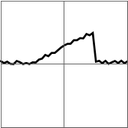
\includegraphics[width=\textwidth]{nabor1_1}
		\end{subfigure} &
		\begin{subfigure}[t]{0.22\textwidth}
			\centering
			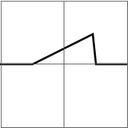
\includegraphics[width=\textwidth]{nabor1_2}
		\end{subfigure} &
		\begin{subfigure}[t]{0.22\textwidth}
			\centering
			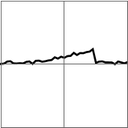
\includegraphics[width=\textwidth]{nabor2_1}
		\end{subfigure} &
		\begin{subfigure}[t]{0.22\textwidth}
			\centering
			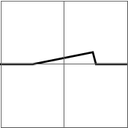
\includegraphics[width=\textwidth]{nabor2_2}
		\end{subfigure} \\
		\multicolumn{2}{c}{\small (a) Тест 1 из набора №1} &
		\multicolumn{2}{c}{\small (d) Тест 1 из набора №2} \\
		
		% Вторая строка изображений
		\begin{subfigure}[t]{0.22\textwidth}
			\centering
			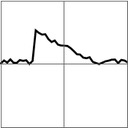
\includegraphics[width=\textwidth]{nabor1_3}
		\end{subfigure} &
		\begin{subfigure}[t]{0.22\textwidth}
			\centering
			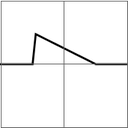
\includegraphics[width=\textwidth]{nabor1_4}
		\end{subfigure} &
		\begin{subfigure}[t]{0.22\textwidth}
			\centering
			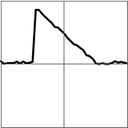
\includegraphics[width=\textwidth]{nabor2_3}
		\end{subfigure} &
		\begin{subfigure}[t]{0.22\textwidth}
			\centering
			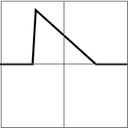
\includegraphics[width=\textwidth]{nabor2_4}
		\end{subfigure} \\
		\multicolumn{2}{c}{\small (b) Тест 2 из набора №1} &
		\multicolumn{2}{c}{\small (e) Тест 2 из набора №2} \\
		
		% Третья строка изображений
		\begin{subfigure}[t]{0.22\textwidth}
			\centering
			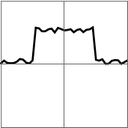
\includegraphics[width=\textwidth]{nabor1_5}
		\end{subfigure} &
		\begin{subfigure}[t]{0.22\textwidth}
			\centering
			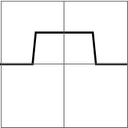
\includegraphics[width=\textwidth]{nabor1_6}
		\end{subfigure} &
		\begin{subfigure}[t]{0.22\textwidth}
			\centering
			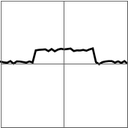
\includegraphics[width=\textwidth]{nabor2_5}
		\end{subfigure} &
		\begin{subfigure}[t]{0.22\textwidth}
			\centering
			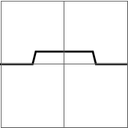
\includegraphics[width=\textwidth]{nabor2_6}
		\end{subfigure} \\
		\multicolumn{2}{c}{\small (c) Тест 3 из набора №1} &
		\multicolumn{2}{c}{\small (f) Тест 3 из набора №2} \\
	\end{tabular}
	\caption{Примеры пар изображений из наборов данных}
	\label{fig:grid_example}
\end{figure}


\newpage




\subsection{Модель}

Для решения задачи очистки зашумленных изображений была выбрана сверточная нейронная сеть (CNN), способная эффективно извлекать пространственные закономерности из изображений. Сверточные нейронные сети хорошо зарекомендовали себя в задачах обработки изображений благодаря их способности автоматически извлекать иерархические признаки с помощью сверток. В данном случае сеть обучается на парах "зашумленное изображение — чистое изображение, чтобы научиться удалять шум.

Архитектура сети состоит из нескольких сверточных слоев и механизмов декодирования для восстановления изображения. Рассмотрим основные компоненты сети:
\begin{itemize}
	\item \textbf{Входной слой:} Принимает изображения размером $128 \times 128$ с одним каналом (градации серого). 
	
	\item \textbf{Сверточные слои:} Используются 4 последовательные свертки с ядром размером $3 \times 3$ и шагом 1. Каждая свертка сопровождается функцией активации \texttt{ReLU}, что позволяет сети эффективно обучаться нелинейным зависимостям. %Параметры инициализируются с применением метода \texttt{He\_Initialization}.
	
	\item \textbf{Уменьшение размерности (MaxPooling):} После нескольких сверточных слоев применяется слой пулинга с окном $2 \times 2$ и шагом 2 для уменьшения размерности карты признаков и сокращения вычислительных затрат.
	
	\item \textbf{Блочная структура (Residual Blocks):} Модель включает несколько остаточных блоков, в которых каждая пара сверточных слоев соединена пропускным соединением (skip connection). Это помогает предотвратить затухание градиента и улучшить обучение на глубоких уровнях.
	
	\item \textbf{Декодирующие слои (Transposed Convolutions):} На этапе восстановления разрешения используются транспонированные свертки с ядром $3 \times 3$, что позволяет увеличить размерность карт признаков и восстановить изображение до исходного размера.
	
	\item \textbf{Выходной слой:} Завершающий сверточный слой с функцией активации \texttt{sigmoid}, который возвращает выходное изображение с диапазоном значений $[0, 1]$.
\end{itemize}

Каждый из этих компонентов обеспечивает извлечение и восстановление признаков изображения, что делает сеть способной эффективно устранять шум.








Для подготовки данных используется функция \texttt{create\_denoising\_dataset()}, которая:
\begin{itemize}
	\item Загружает изображения из указанных папок.
	\item Преобразует изображения в формат $128 \times 128$.
	\item Нормализует данные в диапазон $[0, 1]$.
\end{itemize}
 Для оптимизации используется алгоритм градиентного спуска, который обеспечивает быструю и стабильную сходимость. Функция потерь — среднеквадратичная ошибка.

Таким образом, сеть минимизирует разницу между предсказанным и целевым изображением, что позволяет эффективно удалять шум из изображений.
\lstinputlisting[caption={Модель нейронной сети c использованием TensorFlow}, inputencoding=utf8]{code/Model.py}
\newpage

\section{Анализ результатов}
Для оценки работы алгоритма будем использовать значение функции потерь для различных тестовых примеров. Оценивать будем работу сети как на тестах, которых она училась, так и на двух других тестах из исходного задания. 

Введем величины $\kappa = L_{in} - L_{out}$ и  $\psi =  L_{in} / L_{out}$, где $L_{in}$ --- значение функции потерь на входных данных, $L_{out}$ --- ее значение на результате сети. 

\begin{figure}[!hp] 
	\centering
	\begin{tabular}{cc@{\hspace{1cm}}cc}  
		% Первая строка изображений
		\begin{subfigure}[t]{0.2\textwidth}   
			\centering
			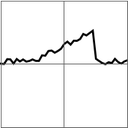
\includegraphics[width=\textwidth]{res_n1_1}  
		\end{subfigure} &
		\begin{subfigure}[t]{0.2\textwidth}   
			\centering
			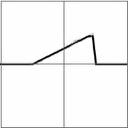
\includegraphics[width=\textwidth]{res_n1_2}  
		\end{subfigure} &
		\begin{subfigure}[t]{0.2\textwidth}   
			\centering
			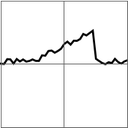
\includegraphics[width=\textwidth]{res_n1_1}  
		\end{subfigure} &
		\begin{subfigure}[t]{0.2\textwidth}   
			\centering
			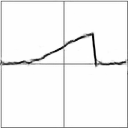
\includegraphics[width=\textwidth]{res_n2_2}  
		\end{subfigure} \\
		\multicolumn{2}{c}{\small 
			\shortstack{(a) Тест 1 для набора №1\\ 
			$L_{in} = 0.0198 , L_{out} = 0.0005$, \\ 
			$\kappa = 0.0193, \psi = $}} &  
		\multicolumn{2}{c}{\small \shortstack{(d) Тест 1  для набора №2 \\ 
				$L_{in} = 0.0198, L_{out} = 0.0107,$\\
				$ \kappa = 0.009, \psi = 1.84$}} \\
		
		% Вторая строка изображений
		\begin{subfigure}[t]{0.2\textwidth}   
			\centering
			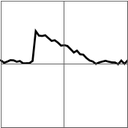
\includegraphics[width=\textwidth]{res_n1_3}  
		\end{subfigure} &
		\begin{subfigure}[t]{0.2\textwidth}   
			\centering
			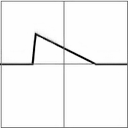
\includegraphics[width=\textwidth]{res_n1_4}  
		\end{subfigure} &
		\begin{subfigure}[t]{0.2\textwidth}   
			\centering
			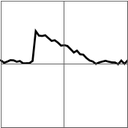
\includegraphics[width=\textwidth]{res_n1_3}  
		\end{subfigure} &
		\begin{subfigure}[t]{0.2\textwidth}   
			\centering
			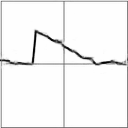
\includegraphics[width=\textwidth]{res_n2_4}  
		\end{subfigure} \\
		\multicolumn{2}{c}{\small \shortstack{(b) Тест 2  для набора №1\\
				 $L_{in} =0.0205 , L_{out} = 0.0002$ \\ 
				 $\kappa = 0.0204, \psi = $ }} &  
		\multicolumn{2}{c}{\small \shortstack{(e) Тест 2 для набора №2 \\ 
				$L_{in} = 0.0205, L_{out} = 0.0118,$\\
				$ \kappa = 0.0087, \psi = 1.73$}} \\
		
		% Третья строка изображений
		\begin{subfigure}[t]{0.2\textwidth}   
			\centering
			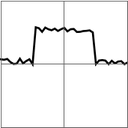
\includegraphics[width=\textwidth]{res_n1_5}  
		\end{subfigure} &
		\begin{subfigure}[t]{0.2\textwidth}   
			\centering
			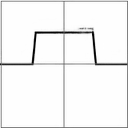
\includegraphics[width=\textwidth]{res_n1_6}  
		\end{subfigure} &
		\begin{subfigure}[t]{0.2\textwidth}   
			\centering
			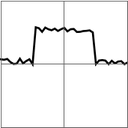
\includegraphics[width=\textwidth]{res_n1_5}  
		\end{subfigure} &
		\begin{subfigure}[t]{0.2\textwidth}   
			\centering
			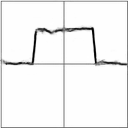
\includegraphics[width=\textwidth]{res_n2_6}  
		\end{subfigure} \\
		\multicolumn{2}{c}{\small \shortstack{(c) Тест 3 для набора №1 \\
				 $L_{in} = 0.0195, L_{out} = 0.0004,$\\
				 $ \kappa = 0.0191, \psi = $}} &  
		\multicolumn{2}{c}{\small \shortstack{(c) Тест 3  для набора №2\\ 
				$L_{in} = 0.0195, L_{out} = 0.0109,$\\
				$ \kappa = 0.0086, \psi = 1.78$}} \\
		
		% Четвертая строка изображений
		\begin{subfigure}[t]{0.2\textwidth}   
			\centering
			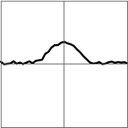
\includegraphics[width=\textwidth]{res_n1_7}  
		\end{subfigure} &
		\begin{subfigure}[t]{0.2\textwidth}   
			\centering
			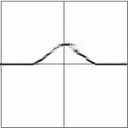
\includegraphics[width=\textwidth]{res_n1_8}  
		\end{subfigure} &
		\begin{subfigure}[t]{0.2\textwidth}   
			\centering
			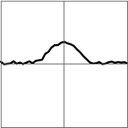
\includegraphics[width=\textwidth]{res_n1_7}  
		\end{subfigure} &
		\begin{subfigure}[t]{0.2\textwidth}   
			\centering
			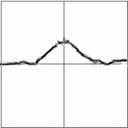
\includegraphics[width=\textwidth]{res_n2_8}  
		\end{subfigure} \\
		\multicolumn{2}{c}{\small \shortstack{(b) Тест 4  для набора №1 \\
				 $L_{in} =0.0205 , L_{out} = 0.0002,$\\
				 $ \kappa = 0.0204, \psi = $}} &
		\multicolumn{2}{c}{\small \shortstack{(e) Тест 4  для набора №2 \\
				 $L_{in} = 0.0205, L_{out} = 0.0118,$\\
				 $ \kappa = 0.006, \psi = $}} \\  
	\end{tabular}
	\caption{Результаты тестов} 
	\label{result}
\end{figure}
\newpage
\begin{figure}[!hp] 
	\centering
	\begin{tabular}{cc@{\hspace{1cm}}cc}  
		% Первая строка изображений
		\begin{subfigure}[t]{0.2\textwidth}   
			\centering
			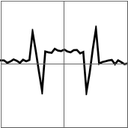
\includegraphics[width=\textwidth]{res_n1_9}  
		\end{subfigure} &
		\begin{subfigure}[t]{0.2\textwidth}   
			\centering
			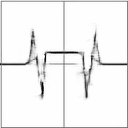
\includegraphics[width=\textwidth]{res_n1_10}  
		\end{subfigure} &
		\begin{subfigure}[t]{0.2\textwidth}   
			\centering
			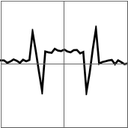
\includegraphics[width=\textwidth]{res_n1_9}  
		\end{subfigure} &
		\begin{subfigure}[t]{0.2\textwidth}   
			\centering
			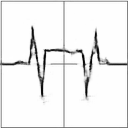
\includegraphics[width=\textwidth]{res_n2_10}  
		\end{subfigure} \\
		\multicolumn{2}{c}{\small \shortstack{(a) Тест 5  для набора №1 \\
				 $L_{in} = 0.0218 , L_{out} = 0.0005$, \\
				  $\kappa = 0.0193, \psi = $}} &  
		\multicolumn{2}{c}{\small \shortstack{(d) Тест 5  для набора №2 \\ 
				$L_{in} = 0.0218, L_{out} = 0.0037,$\\
				$ \kappa = 0.0181, \psi = $}} \\
	\end{tabular}
	\caption{Результаты тестов} 
	\label{result}
\end{figure}


На основе приведенных результатов можно сделать общий вывод о высокой эффективности работы разработанной нейронной сети. Значение функции потерь на выходе модели ($L_{out}$) значительно ниже, чем на входе ($L_{in}$) во всех тестах, что указывает на успешное подавление шума и корректную обработку численного решения. Величина $\kappa = L_{in} - L_{out}$ положительна во всех тестах, демонстрируя улучшение качества данных после обработки сетью. Например, для теста 2 величина $\kappa$ составляет $0.0204$, что свидетельствует о существенном снижении ошибки. 

Стабильность работы модели подтверждается тем, что значения $\kappa$ находятся в пределах одинакового порядка ($\approx 0.018 - 0.020$) для всех тестов, что говорит о надежности сети при обработке различных входных данных. Однако стоит отметить, что в тестах 4 и 5 наблюдаются более высокие значения $L_{out}$ ($0.0037$ и $0.0118$ соответственно). Это происходит из-за того, что эти фигуры не были включены в обучающую выборку. 

Таким образом, можно сделать вывод, что модель эффективно справляется с задачей подавления шума на численных решениях уравнения переноса, что подтверждается значительным снижением функции потерь и стабильностью результатов на различных тестах.

\section{Актуальность и перспективы задачи}
Задача устранения шума с численных решений уравнения переноса с использованием нейронных сетей является актуальной в контексте широкого применения численных методов в моделировании физических процессов. Уравнение переноса описывает разнообразные явления, такие как распространение тепла, движение жидкостей и газов, а также перенос загрязняющих веществ в атмосфере и гидросфере. Однако численные методы при использовании приближённых схем часто сопровождаются возникновением численного шума, артефактов и дисперсии, что снижает точность моделирования и усложняет дальнейший анализ.

Использование сверточных нейронных сетей для устранения шума обладает рядом преимуществ:
\begin{itemize}
	\item \textbf{Автоматическое устранение артефактов}: Нейронные сети могут обучаться выделять полезные сигналы и игнорировать шум без ручной настройки параметров фильтрации. 
	\item \textbf{Высокая гибкость}: Сеть может адаптироваться к различным типам шума и условиям моделирования, что делает её универсальным инструментом для работы с численными данными. Автоматическое улучшение качества численного решения уменьшает потребность в дополнительных фильтрационных процедурах, что ускоряет процесс анализа. 
\end{itemize}

%Перспектив применения множество. Использование нейронных сетей для обработки численных решений может найти применение в аэродинамическом моделировании, гидродинамике и теплопередаче, где точность данных играет ключевую роль. Обученные модели могут использоваться для коррекции численных решений в реальном времени, что позволит применять менее ресурсоемкие численные схемы без потери точности.
Таким образом, разработка и внедрение методов устранения шума на основе нейронных сетей открывает новые перспективы для численного моделирования сложных процессов, позволяя достигать более высокой точности и надежности результатов.





\section-{Заключение}

В данной работе рассмотрена задача устранения шума с численных решений уравнения переноса с помощью нейронных сетей. Применение современных методов машинного обучения, в частности сверточных нейронных сетей, позволило разработать эффективный подход к улучшению точности численных решений. 

В ходе исследования реализована архитектура сверточной нейронной сети, способная обрабатывать дискретные численные данные, подавляя шум и восстанавливая исходную структуру решения. Подробно рассмотрены ключевые этапы построения модели, включая выбор слоев, функции активации, методы оптимизации и обучение сети на синтетических данных.

Анализ полученных результатов продемонстрировал, что предложенная модель способна эффективно устранять шум и значительно улучшать качество численных решений уравнения переноса. Это подтверждает перспективность использования нейросетевых подходов в задачах численного моделирования.

Применение разработанного метода может найти широкий отклик в различных научных и инженерных областях, где требуется высокоточная обработка численных данных. Перспективы дальнейших исследований включают оптимизацию архитектуры сети, адаптацию модели для различных типов уравнений и развитие методов реального времени для обработки больших объемов данных.

 


\clearpage
\begin{thebibliography}{1}

\bibitem{1} Галанин М.П., Савенков Е.Б. Методы численного анализа математических моделей. М.: Изд-во МГТУ им. Н.Э. Баумана. 2018. 592 с.


\bibitem{2} Tariq Rashid Make Your Own Neural Network // CreateSpace Independent Publishing Platform; 1st edition SAND96-0583 (March 31, 2016)


\bibitem{3} Глубокое обучение / Николенко С., Кадурин А., Архангельская Е. - СПб. : Питер, 2022. - 476 с. : рис. - (Библиотека программиста). - Библиогр.: с. 451-476. - ISBN 978-5-4461-1537-2.


\bibitem{4} Элементы математической теории машинного обучения : учебное пособие для вузов / Вьюгин В. В. ; Моск. физико-техн. ин-т (гос. ун-т), РАН. Ин-т проблем передачи информации им. А. А. Харкевича. - М. : МФТИ - ИППИ РАН, 2010. - 231 с. - Библиогр.: с. 229-231. - ISBN 978-5-7417-0339-7.


\bibitem{5} Вьюгин В.В. “Математические основы машинного обучения и прогнозирования” М.: 2013, 2018 - 484 с.


\bibitem{6} Машинное обучение и TeпsorFlow. - СПб.: Питер, 2019. - 336 с.: ил. - (Серия «Библиотека программиста»). ISBN 978-5-4461-0826-8


\bibitem{7} Нейронные сети: полный курс, 2-е издание. : Пер. с англ. --- М.: Издательский дом "Вильямс", 2006. --- 1104 с.: 1104с.:ил. Парал.тит.англ. ISBN 5-8459-0890-6(рус.)


\bibitem{8} Теория и практика машинного обучения : учебное пособие /В. В. Воронина, А. В. Михеев, Н. Г. Ярушкина, К. В. Святов. –Ульяновск : УлГТУ, 2017. – 290 с


\bibitem{9} Глубокое обучение на Python / Шолле Франсуа — СПб.: Питер, 2018. — 400 с.: ил. — (Серия «Библиотека программиста»).ISBN 978-5-4461-0770-4

\bibitem{10} Искусственные нейронные сети и приложения: учеб. пособие /Ф.М. Гафаров, А.Ф. Галимянов. – Казань: Изд-во Казан. ун-та, 2018. –121 с.




\end{thebibliography}

\end{document} 